

% -- % -- % -- % -- % -- %
% -- % -- % -- % -- % -- %

% This example file for NIH submissions was originally written
% by Bruce Donald (http://www.cs.duke.edu/brd/).
% 
% You may freely use, modify and/or distribute this file.
% 
\documentclass[11pt]{nih}
%\documentclass{article}
%\documentclass[12pt]{article}%
% last revision:
\def\mydate{2005-06-09 13:58:03 brd}


%%%%%%% Two column control
\newif\ifdotwocol
\dotwocoltrue  % two col
%\dotwocolfalse  % one col
\long\def\twocol#1#2{\ifdotwocol{#1}\else{#2}\fi}
%%%%%%%

\def\mybeforeequation{\footnotesize}
%\def\mybeforeequation{\small}
%\def\mybeforeequation{}

\def\myafterequation{\renewcommand\baselinestretch{1.1}}
%\def\myafterequation{}

%%%%%%%%%%%%%%%%
%%%%%%%%%%%%%%%%

\def\citeusmark{$^{\textstyle \star}$}
\def\citeus#1#2{\cite{#1}}

\def\crow#1#2{#2}

%\usepackage{denselists}
%\usepackage{scaledfullpage}
\usepackage[dvips]{graphicx}
\usepackage{color}
\usepackage{boxedminipage}
\usepackage{amsfonts}
\usepackage{amsmath}
\usepackage{url}
%\usepackage{times}
%\usepackage{nih}		% PHS 398 Forms
%\usepackage{nihblank}		% For printing on Blank PHS 398 Forms
%\usepackage{confidential}

\def\Paper{grant application}
\def\paper{application}
\def\refappendix{Sec.}

\def\poster{(Poster)}

%Note from brd
\long\def\todo#1{{\bf{To do:}} #1}
%\long\def\todo#1{}
\def\ICRA{IEEE International Conference on Robotics and Automation (ICRA)}

\long\def\squeezable#1{#1}

%\def\a5{$\alpha_{_5}$

\def\a5{5}

%\def\mycaptionsize{\normalsize}
%\def\mycaptionsize{\small}
%\def\mycaptionsize{\small}
\def\mycaptionsize{\footnotesize}
\def\mycodesize{\footnotesize}
\def\myeqnsize{\small}

\def\sheading#1{{\bf #1:}\ }
\def\sheading#1{\subsubsection{#1}}
%\def\sheading#1{\bigskip {\bf #1.}}

\def\ssheading#1{\noindent {\bf #1.}\ } 

\newtheorem{hypothesis}{Hypothesis}
\long\def\hyp#1{\begin{hypothesis} #1 \end{hypothesis}}

\def\cbk#1{[{\em #1}]}

\def\R{\mathbb{R}}
\def\midv{\mathop{\,|\,}}
\def\Fscr{\mathcal{F}}
\def\Gscr{\mathcal{G}}
\def\Sscr{\mathcal{S}}
\def\set#1{{\{#1\}}}
\def\edge{\!\rightarrow\!}
\def\dedge{\!\leftrightarrow\!}
\newcommand{\EOP}{\nolinebreak[1]~~~\hspace*{\fill} $\Box$\vspace*{\parskip}\vspace*{1ex}}
%my way of doing starred references
\newcommand{\mybibitem}[1]{\bibitem{#1} 
\label{mybiblabel:#1}}
\newcommand{\BC}{[}
\newcommand{\EC}{]}
\newcommand{\mycite}[1]{\ref{mybiblabel:#1}\nocite{#1}}
\newcommand{\starcite}[1]{\ref{mybiblabel:#1}\citeusmark\nocite{#1}}


\def\degree{$^\circ$}
\def\R{\mathbb{R}}
\def\Fscr{\mathcal{F}}
\def\set#1{{\{#1\}}}
\def\edge{\!\rightarrow\!}
\def\dedge{\!\leftrightarrow\!}

\long\def\gobble#1{}
\def\Jigsaw{{\sc Jigsaw}}
\def\ahelix{\ensuremath{\alpha}-helix}
\def\ahelices{\ensuremath{\alpha}-helices}
\def\ahelical{$\alpha$-helical}
\def\bstrand{\ensuremath{\beta}-strand}
\def\bstrands{\ensuremath{\beta}-strands}
\def\bsheet{\ensuremath{\beta}-sheet}
\def\bsheets{\ensuremath{\beta}-sheets}
\def\hone{{\ensuremath{^1}\rm{H}}}
\def\htwo{{$^{2}$H}}
\def\cthir{{\ensuremath{^{13}}\rm{C}}}
\def\nfif{{\ensuremath{^{15}}\rm{N}}}
\def\hn{{\rm{H}\ensuremath{^\mathrm{N}}}}
\def\hnone{{\textup{H}\ensuremath{^1_\mathrm{N}}}}
\def\ca{{\rm{C}\ensuremath{^\alpha}}}
\def\catwel{{\ensuremath{^{12}}\rm{C}\ensuremath{^\alpha}}}
\def\ha{{\rm{H}\ensuremath{^\alpha}}}
\def\cb{{\rm{C}\ensuremath{^\beta}}}
\def\hb{{\rm{H}\ensuremath{^\beta}}}
\def\hg{{\rm{H}\ensuremath{^\gamma}}}
\def\dnn{{\ensuremath{d_{\mathrm{NN}}}}}
\def\dan{{\ensuremath{d_{\alpha \mathrm{N}}}}}
\def\jconst{{\ensuremath{^{3}\mathrm{J}_{\mathrm{H}^{\mathrm{N}}\mathrm{H}^{\alpha}}}} }
\def\cbfb{{CBF-$\beta$}}

\newtheorem{defn}{Definition}
\newtheorem{claim}{Claim}

  \gobble{
  \psfrag{CO}[][]{\colorbox{white}{C}}
  \psfrag{OO}[][]{\colorbox{white}{O}}
  \psfrag{CA}[][]{\colorbox{white}{\ca}}
  \psfrag{HA}[][]{\colorbox{white}{\ha}}
  \psfrag{CB}[][]{\colorbox{white}{\cb}}
  \psfrag{HB}[][]{\colorbox{white}{\hb}}
  \psfrag{HN}[][]{\colorbox{white}{\hn}}
  \psfrag{N15}[][]{\colorbox{white}{\nfif}}
  \psfrag{dnn}[][]{\dnn}
  \psfrag{dan}[][]{\dan}
  \psfrag{phi}[][]{$\phi$}
  }

\newenvironment{closeenumerate}{\begin{list}{\arabic{enumi}.}{\topsep=0in\itemsep=0in\parsep=0in\usecounter{enumi}}}{\end{list}}
\def\CR{\hspace{0pt}}      % ``invisible'' space for line break



\newif\ifdbspacing
%\dbspacingtrue % For double spacing
\dbspacingfalse % For normal spacing

\ifdbspacing
 \doublespacing
 \newcommand{\capspacing}{\doublespace\mycaptionsize}
\else
 \newcommand{\capspacing}{\mycaptionsize}
\fi

\def\rulefigure{\smallskip\hrule}

% \def\codesize{\normalsize}
\def\codesize{\small}

% Can use macros \be, \ee, \en as shortcuts
% for \begin{enumerate}, \end{enumerate}, \item
% respectively.

\def\be{\begin{enumerate}}  % Begin Enumerate
\def\ee{\end{enumerate}}   % End Enumerate
\def\en{\item}        % ENtry (item)
\def\bi{\begin{itemize}}   % Begin Itemize
\def\ei{\end{itemize}}    % End Itemize
\def\bv{\begin{verbatim}}  % Begin Verbatim
\def\ev{\end{verbatim}}   % End Verbatim

\def\matlab{{\sc matlab} }
\def\amber{{\sc amber} }
\def\KS{{$K^*$}}
\def\KSM{{K^*}} % K-Star Math
\def\KSTM{{\tilde{K}^*}} % K-Star Tilde Math (appx K*)
\def\KOP{{$K^{\dagger}_{o}$}} % K-Star Optimal partial
\def\KOPM{{K^{\dagger}_{o}}} % K-Star Optimal partial Math
\def\KP{{$K^{\dagger}$}} % K-Star partial
\def\KPM{{K^{\dagger}}} % K-Star partial Math
\def\KTPM{{\tilde{K}^{\dagger}}} % K-Star Tilde partial Math
\def\KD{{$K_{_D}$}}
\def\KA{{$K_{_A}$}}
\def\qpM{{q_{_P}}}
\def\qlM{{q_{_L}}}
\def\qplM{{q_{_{PL}}}}
\def\qSplM{{q^*_{_{PL}}}}
\def\KSO{{$K^*_{o}$}} % K-Star Optimal
\def\KSOM{{K^*_{o}}} % K-Star Optimal Math
\def\CBFB{{CBF-$\beta$}}  % Core binding factor beta
\def\argmin{\mathop{\mathrm{argmin}}}
\def\rhl#1{{\em \underline{RYAN}: *\{{#1}\}*}}
\def\set#1{{\left\{ #1 \right\}}}
\def\Escr{{\mathcal{E}}}
\def\Jscr{{\mathcal{J}}}
\def\Kscr{{\mathcal{K}}}
\def\th{{$^{{\mathrm{th}}}$}}

\newtheorem{proposition}{Proposition}
\newtheorem{lemma}{Lemma}
\usepackage[width=7.0in, height=9.5in, head=0.0in, foot=0.0in, headsep=0.0in]{geometry}
%% This controls margins. Can't go over width=7.5in, height=10.0in. 
%% top-bottom margins = (11-height)/2 left-right margins = (8.5-width)/2

\usepackage{setspace} % useful in changing vertical spacing temporarily.
%\onehalfspacing
\usepackage{natbib} % more control over how references appear within text.
\bibpunct{[}{]}{,}{n}{}{} % like so.
%% use \citep{ref} instead of \cite{ref} in text.
\usepackage[font=footnotesize,labelfont=bf]{caption}
\usepackage{textgreek}
\usepackage{sectsty} % can change font, size of the section headings. 
\usepackage{wrapfig}
\usepackage{graphicx}
\usepackage{sidecap} %required for side captions
\setlength{\parskip}{0pt}
\setlength{\parsep}{0pt}
\setlength{\headsep}{0pt}
 \setlength{\topskip}{0pt}
\setlength{\topmargin}{0pt}
\setlength{\topsep}{0pt}
 \setlength{\partopsep}{0pt}
\sectionfont  {\fontsize{11pt}{3}\usefont{OT1}{phv}{b}{sc}\selectfont}
\subsectionfont {\fontsize{11pt}{3}\usefont{OT1}{phv}{b}{n}\selectfont}
%\subsubsectionfont{\fontsize{11pt}{\itshape\underline}{3}\usefont{OT1}{phv}{m}{n}\selectfont} 
\subsubsectionfont{\normalfont\large\itshape\underline}


\renewcommand{\thesection}{\Alph{section}} % so that section headings use A B C instead 1 2 3
\renewcommand{\baselinestretch}{1}

\renewcommand\refname{\section{Literature Cited} \vspace{-1em}} 
%% This changes ``Reference'' to ``Literature Cited''. 

\newcommand{\inden}[1]{\mbox{} \hspace{#1} } % Force horizontal spaces. 
\usepackage[compact]{titlesec}
\titlespacing{\section}{0pt}{*0}{*0}
 \titlespacing{\subsection}{0pt}{*0}{*0}
\titlespacing{\subsubsection}{0pt}{*0}{*0}


\begin{document}


\bigskip

\appendix 

%\mydate

\setcounter{page}{20} % or whatever



% -- % -- % -- % -- % -- %
% -- % -- % -- % -- % -- %
\section{Post-submission Materials}
\par The COVID-19 pandemic has severely impacted the ability to conduct bench research at academic institutions around the world. At the College of Staten Island,  reseach activity was stopped in March 2020 and the return to research was prioritized for faculty with external funding beginning in August 2020. My laboratory, which was not externally funded, reopened in October 2020, graduate students were permitted to resume limited activity in my lab in March 2021, and undergraduates will resume activity in June 2021. The pause in research activity has resulted in the limited ability to contribute preliminary data to this R15 proposal, and has thus neccesitated this one page post-submission document.
\par The accompanying R15 proposal was built upon previous evdence from our lab that the African naked mole-rat (NM-R) has an enhanced vulnerability to epileptic seizures due, in part, to a variant in the KCC2 gene, which determines neuronal chloride concentration and thus GABA efficacy. The lack of seizure activity reported in this species, along with our demonstration that nest-oriented behavior is their dominant behavior, and our finding that nest conditions suppress seizure susceptibility in NM-R indicate that NM-R overcome their vulnerability through social and environmental factors in the colony nest. Studying the factors which reduce seizure vulnerability in NM-R may yeild new approaches towards treating and preventing seizures in other animals, including humans, particularly those who suffer from epilepsy and have the same loss of function KCC2 variant as NM-R. Therefore, the current proposal is  designed to test the central hypothesis that social and environmental factors in the colony nest, specifically oxytocin and carbon dioxide, enhance KCC2 membrane stability and GABAergic inhibition in the adult NM-R. 
\par While it has been known for some time that carbon dioxide can supress seizure activity \cite{petroianu_2020_singultus}, and we have demonstrated that nest lovels of carbon dioxide can suppress seizures in NM-R \cite{zions_2020_nest}, the neuronal mechanisms driving this effect are not well understood. In the current R15 proposal, we will  test whether enhanced carbon dioxide comensates for the NM-R KCC2 impairment by increasing membrane stabilization of KCC2, specifically through phosphorylation at the ser940 locus.  The R15 proposal includes preliminary data to demonstrate antibody specificity for phosphorylated ser940 KCC2 in NM-R.
\par The hypothesis that oxytocin (OXT) can also supress seizure activity has less support in the extant literature. Unlike carbon dioxide, OXT has already been demonstrated to increase KCC2 membrane stabilization through phosphorylation at the ser940 locus \cite{leonzino_2016_timing}.  This likely plays an important role in the developmental regulation of GABA efficacy, particularly at birth \cite{tyzio_2006_maternal}, but the potential role for this mechanism of oxytocin to inhibit seizure activity has not yet been tested. Previous evidence of OXT's effects on seizure susceptibility has been mixed.  OXT has been shown to reduce seizures in newborn rats following perinatal asphyxia \cite{panaitescu_2018_oxytocin} or in 2-3 month old rats following pentylentetrazol \cite{erbas_2013_oxytocin}, and in 2 month old mice with heterozygous deletion of the gene regulating the\textit{Scn1a} voltage-gated sodium channel \cite{wong_2021_nanoparticle}.  Yet,  OXT has been shown to exacerbate pentylentetrazol seizures in 3 month old mice through activation of vasopressin receptors \cite{loyens_2012_proconvulsive}. These inconsistencies may reflect interactions of species, age, and source of seizure activity. Perhaps the seizure-supression activity of OXT is strongest under conditions of seizure vulnerability.  That is, a typical adult brain, which has reached a ceiling for KCC2-induced neuronal chloride extrusion, may not benefit from OXT treatment.
\par Our preliminary analysis of NM-R hippocampal OXT receptor density, shown in the proposal, indicates a consistent level of receptor which is independent of social role in the NM-R. This, coupled with our demonstration of in impairment in KCC2-based neuronal chloride extrustion \cite{zions_2020_nest}, indicates that the NM-R brain is primed to benefit from the KCC2-enhancing propoerties of OXT \cite{leonzino_2016_timing} to reduce epileptiform activity. To test this, we measured the effect of the selective OXT receptor agonist proposed for use in the proposal (TGOT, 200 nM) to reduce spontaneous epileptiform activity recorded in adult NM-R hippocampal slices. 
\begin{SCfigure}[1][!h].
 \centering
 \includegraphics[width=0.5\textwidth]{Fig2D_new.png}
 \caption{\textbf{Left.} NM-R \textit{in vitro} hippocampal recordings demonstrate periodic epileptiform burst discharges under routine slice recording conditions.  When the carbogen is changed to 100\% O\textsubscrip{2} and bicarbonate in the ACSF is replaced with HEPES, the loss of CO\textsubscript{2} causes an increase in the frequency of the epileptiform burst discharge, consistent with increased excitability. \textbf{Right.}  Analysis of teh burst frequency following removal of CO\textsubscript{2} from the slice shows a 20\% increase in burst frequency in 5 slices (from 3 animals).  This increase was significant when rat burst frequencies were compared with a t-test (\textu{p}<0.05) }
\end{SCfigure}
\par We have observed previously that NM-R hippocampal slices, prepared under typical \textit{in vitro} conditions, exhibit spontaneous epileptiform burst discharges in the pyramidal cell layer of area CA3 \cite{zions_2020_nest}, similar to what we have observed previously in chronic epileptic adult rats \cite{McCloskey2011-sm}. These epileptiform bursts are exacerbated when carbon dioxide is removed from the NM-R slice by replacing the carbogen gas (95\% O\textsubscript{2}, 5\%CO\textsubcript{2}) with 100\% O\textsubscript{2}, and replacing bicarbonate in the buffer with HEPES (Figure 1), supporting the role of carbon dioxide to supress seizure activity. Addition of the  GABA\textsubscript{A} receptor agonist isoguvacine to the slice also, paradoxically, exacerbates epileptiform activity (Figure 2), likely due, in part, to the KCC2 missense mutation in this species.
\begin{SCfigure}[1][!h].
 \centering
 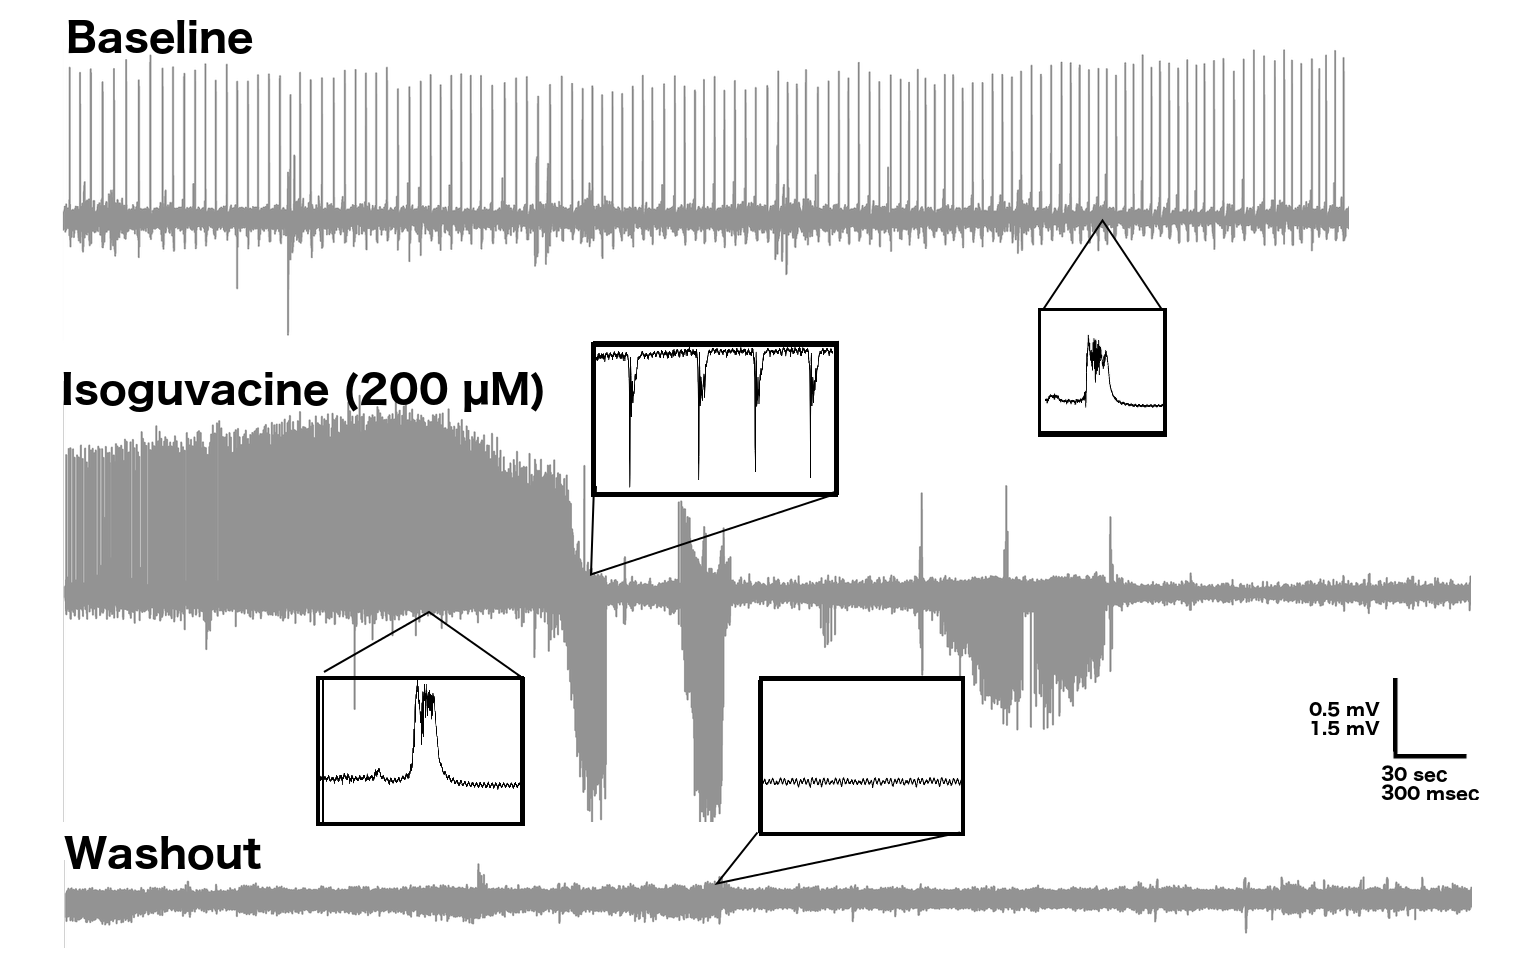
\includegraphics[width=0.5\textwidth]{isoguvacine.png}
 \caption{Baseline recording from hippocampal area CA3 under standard conditions showing epileptiform bursts.  When the GABA\textsubscript {A} agonist isoguvacine (200 \textmu M) was added to the perfusate, slices  increased their bursting activity and developed spreading depression in all slices tested (n=3 slices from 3 animals), indicating an excitatory response to GABA\textsubscript {A} receptor activation.  From \cite{zions_2020_nest}}
\end{SCfigure}
\par To test whether OXT receptor activation suppresses epileptiform activity in the NM-R slice, we applied the selective OXT receptor agonist Thr\textsuperscript{4},Gly\textsuperscript{7}-oxytocin (TGOT) to NM-R slices with epiletiform activity.  Figure 3 shows the robust suppression of epileptiform events we observed in response to 200 200 nM TGOT. This is the dose and method of application outlined in experiment 1.1 of the proposal. The TGOT suppression of epileptiform activity did not readily wash upon returning the slices to normal ASCF for 30 minutes, indicating potential downstream transcription; potentially KCC2 membrane stabilization as hypothesized in the proposal. To test whether GABA enhancement has occurred following TGOT treatment, we again administered isoguvacine following TGOT and a 30 minute wash period.  In this condition isoguvacine further reduced activity in the slice, consistent with a typical GABAergic effect, indicating the OXT receptor activation may "rescue" GABAergic function in the NM-R brain. 
\par Although these data are still preliminary, and proper controls must be performed, they provide support for our central hypothesis that social and environmental factors in the colony nest, specifically oxytocin and carbon dioxide, enhance KCC2 membrane stability and GABAergic inhibition in the adult NM-R.  With the requested funding, we hope to properly test this hypothesis and pave the way to new approaches in the prevention and treatment of epilepsy and other chloride dysfunction disorders.


% -- % -- % -- % -- % -- %
\newpage
\bibliographystyle{myrefstyle} %unsrt should work, too. copy myrefstyle.bst in the same directory as the .tex file.
\bibliography{ref.bib} % Or wherever you keep your .bib file.

% -- % -- % -- % -- % -- %
\end{document}

